%% Last modified: Time-stamp: <2011-08-04 12:43:05 (srdbadmin)>
\documentclass[letterpaper,review,authoryear,12pt]{article}
\usepackage{amssymb}
\usepackage{pdflscape}
\usepackage{longtable}
\usepackage{graphicx}
\usepackage{paralist}
\usepackage{comment}
\usepackage{color}
\usepackage[left=3cm,top=3cm,right=3cm,bottom=3cm,nohead]{geometry}
\usepackage{booktabs}
\usepackage{url}
\usepackage[none]{hyphenat}  %% no hyphenation, to facilitate conversion to Word
\usepackage{microtype} %% no ligature, to facilitate conversion to Word
\DisableLigatures{encoding = *, family = * }
\usepackage{appendix}

\title{Figures for Supporting Information of the accepted Fish and Fisheries paper August 2011}
\date{\today}

\begin{document}
\renewcommand{\figurename}{Fig. S}
\renewcommand{\tablename}{Table S}

\maketitle

\section{Supplementary figures}
\noindent Figure S1. Entity-relationship diagram


\noindent Figure S2. Contingency table\\ 

\noindent Figure S3. Taxonomic coverage of assessed marine species
present in the RAM Legacy database. The circle located near the middle
of the circular dendrogram represents kingdom Animalia and each
subsequent branching represents a different taxonomic group (Kingdom
to Phylum to Class to Order to Family to Genus to Species). The width
of each line is proportional to the square root of the number of
assessments in the database. The outermost lines represent species and
the number of lines is the number of assessments for each species. The
names of multi-assessment species are not repeated on the outermost
portion of the dendrogram but continue counter-clockwise from the
first entry.  Note that branch lengths are chosen for graphical
purposes and do not convey phylogenetic distance.\\

\noindent Figure S4. ICES Blim\\ 

\noindent Figure S5. Functional groups.\\ 


%\begin{landscape}
.\begin{figure}
\begin{center}
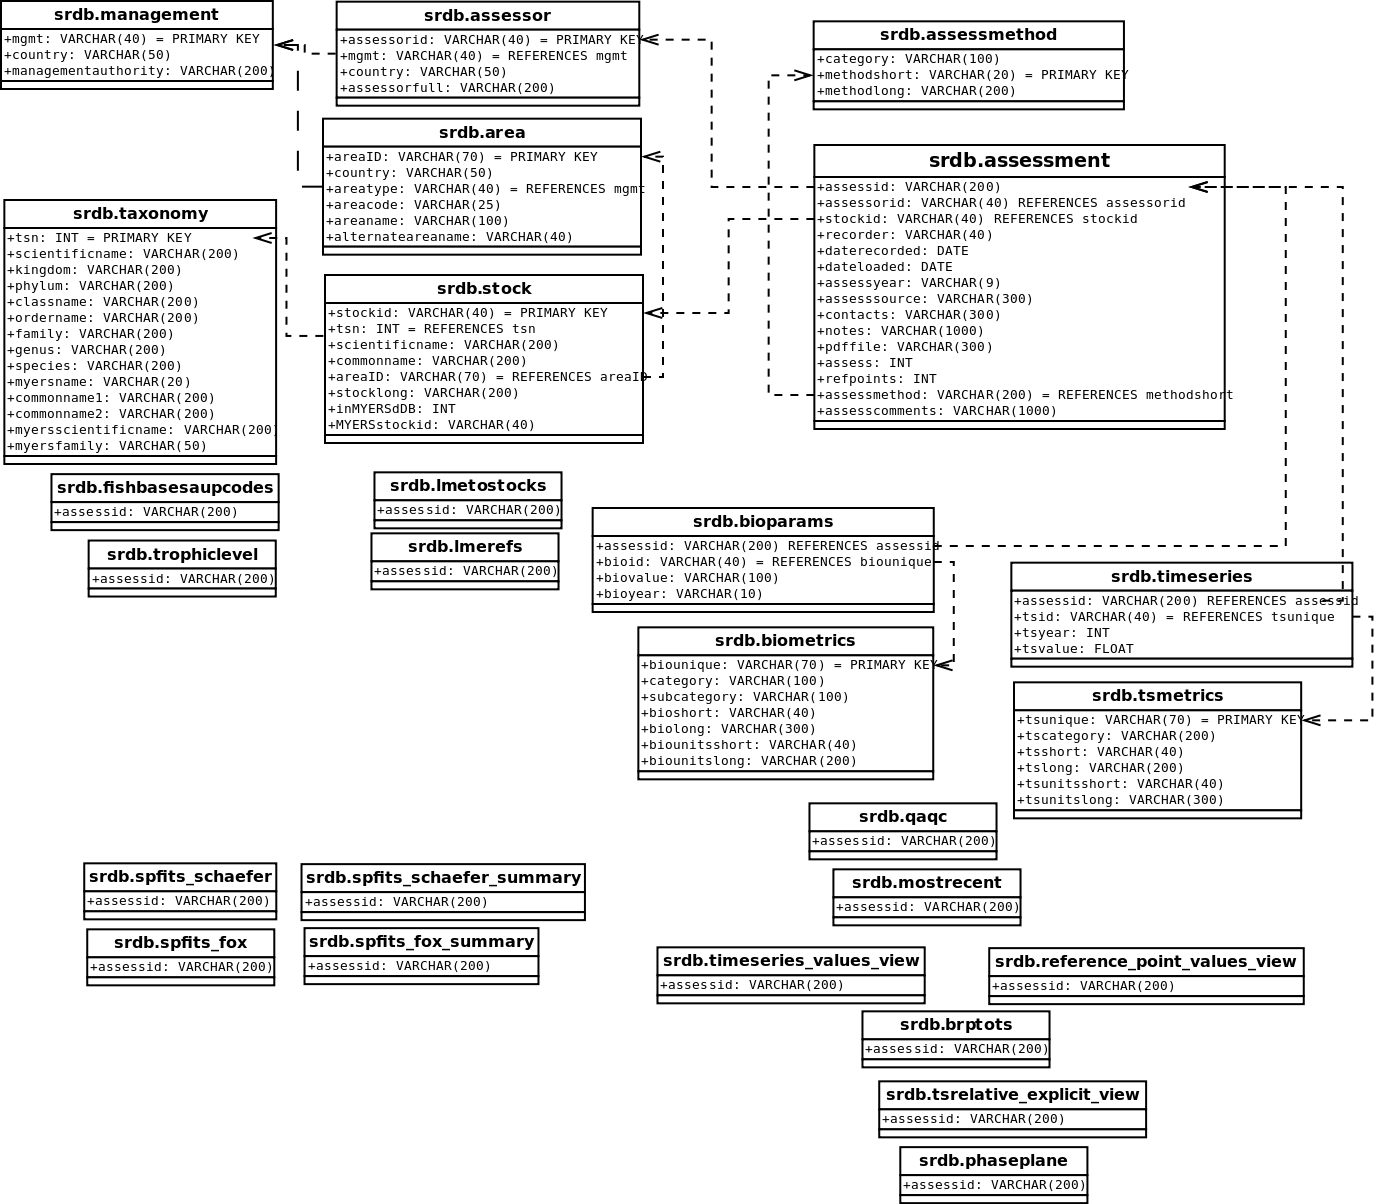
\includegraphics[width=6in]{/home/srdbadmin/srdb/doc/srdb-erd-2011.png}
\end{center}
\caption{ }\label{fig:erd}
\end{figure}
%\end{landscape}

%Comparison of assessment-derived and Schaefer-derived ratios (Figure~\ref{fig:corr}).
\begin{figure}
\begin{center}
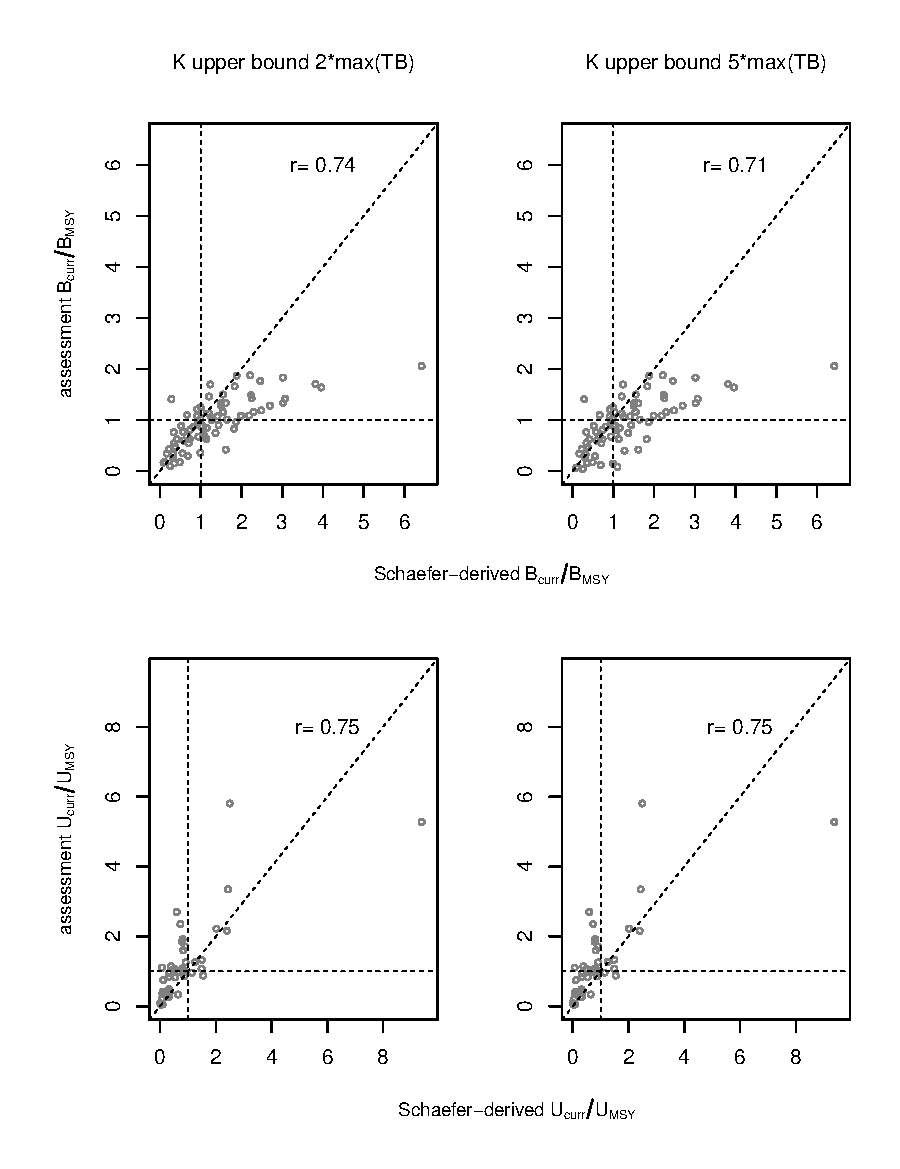
\includegraphics[width=15cm]{/home/srdbadmin/srdb/projects/fishandfisheries/R/PROOFS-final/Schaefer-correlations-Kbounds-comparison.pdf}
\end{center}
\caption{ }\label{fig:corr}
\end{figure}


\begin{figure}
\begin{center}
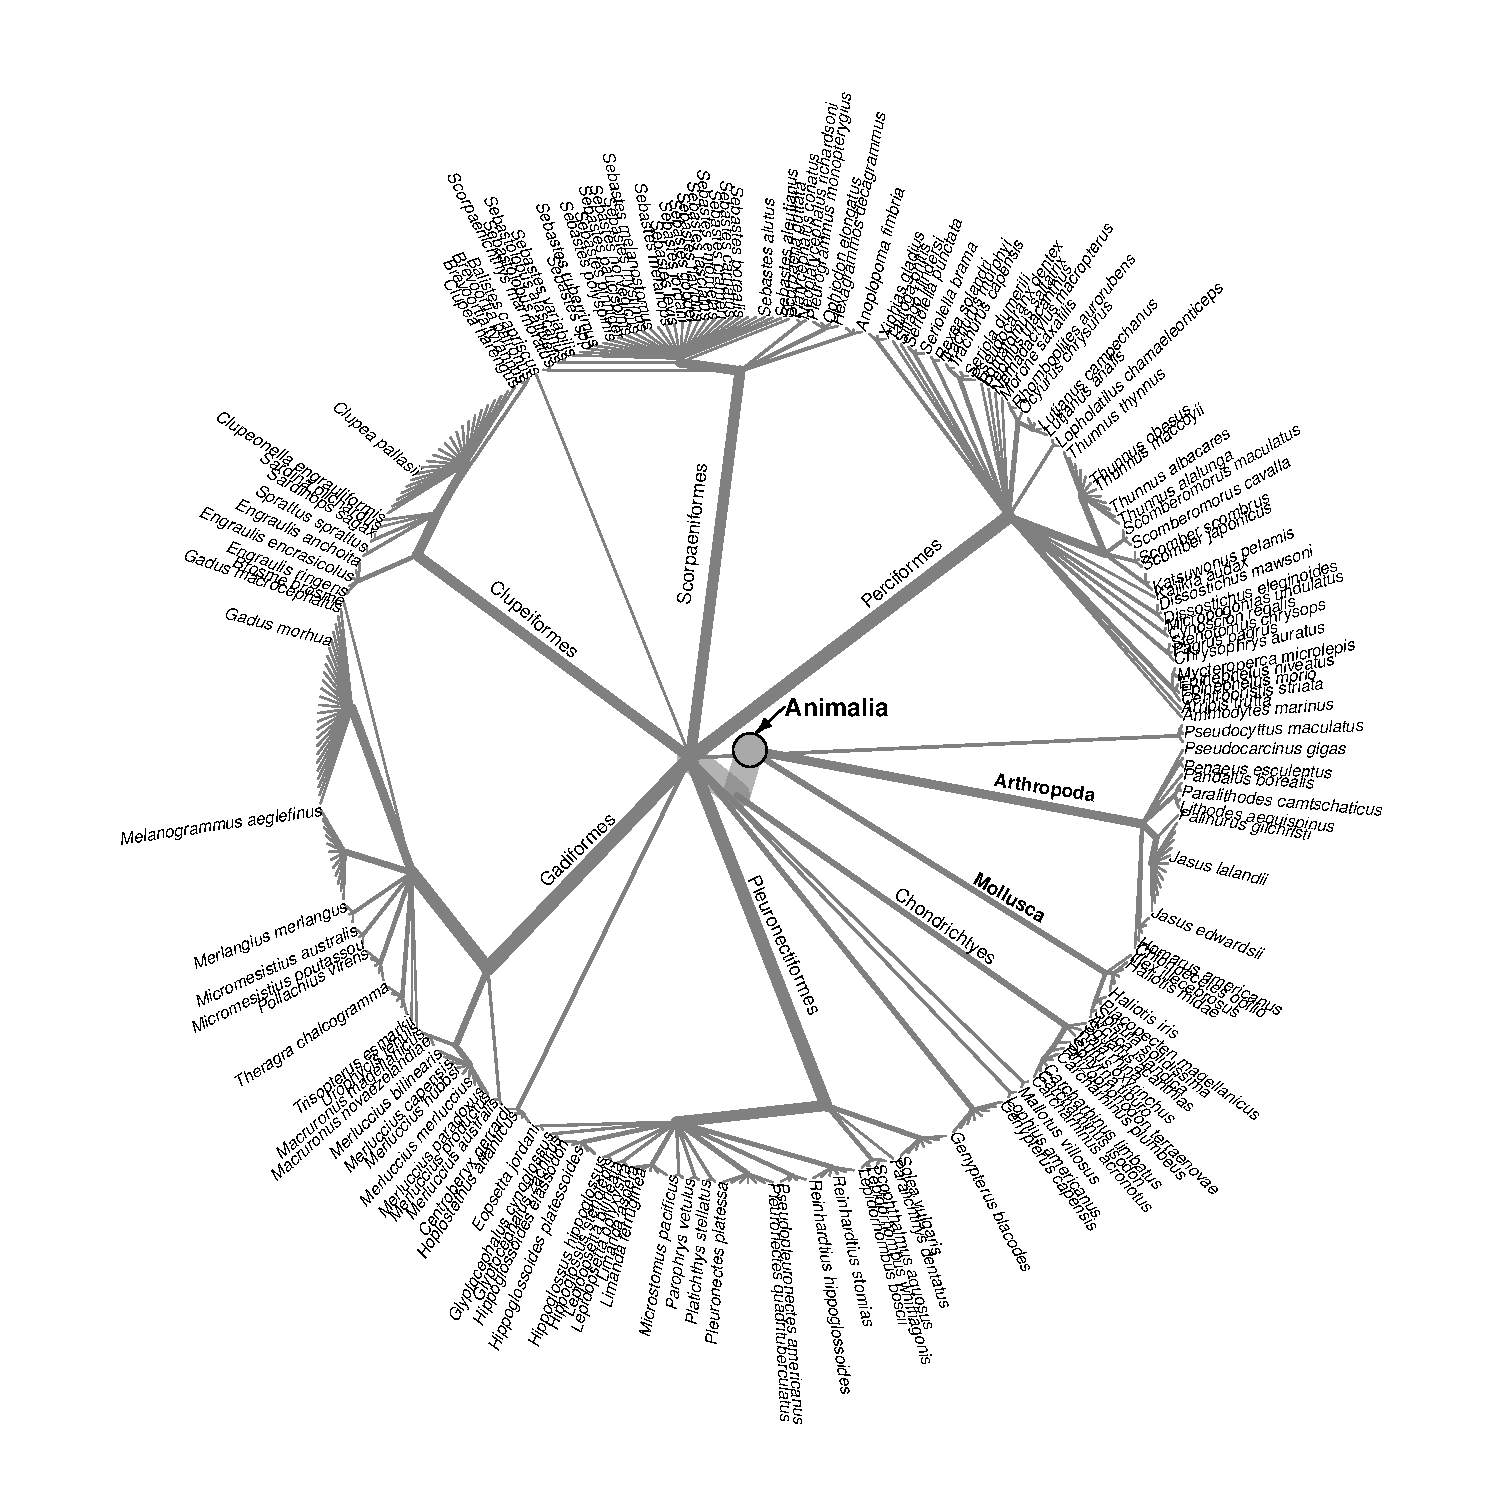
\includegraphics[width=6.5in]{/home/srdbadmin/srdb/projects/fishandfisheries/R/PROOFS-final/srdb-by-assessment.pdf} %taxonomic_coverage_byLME.pdf}
\end{center}
\caption{ }\label{fig:taxo:srdb}
\end{figure}


%Fried egg plot for ICES using SSBlim reference points instead of SSBmsy  (Figure~\ref{fig:icesblim}).
\begin{figure}
\begin{center}
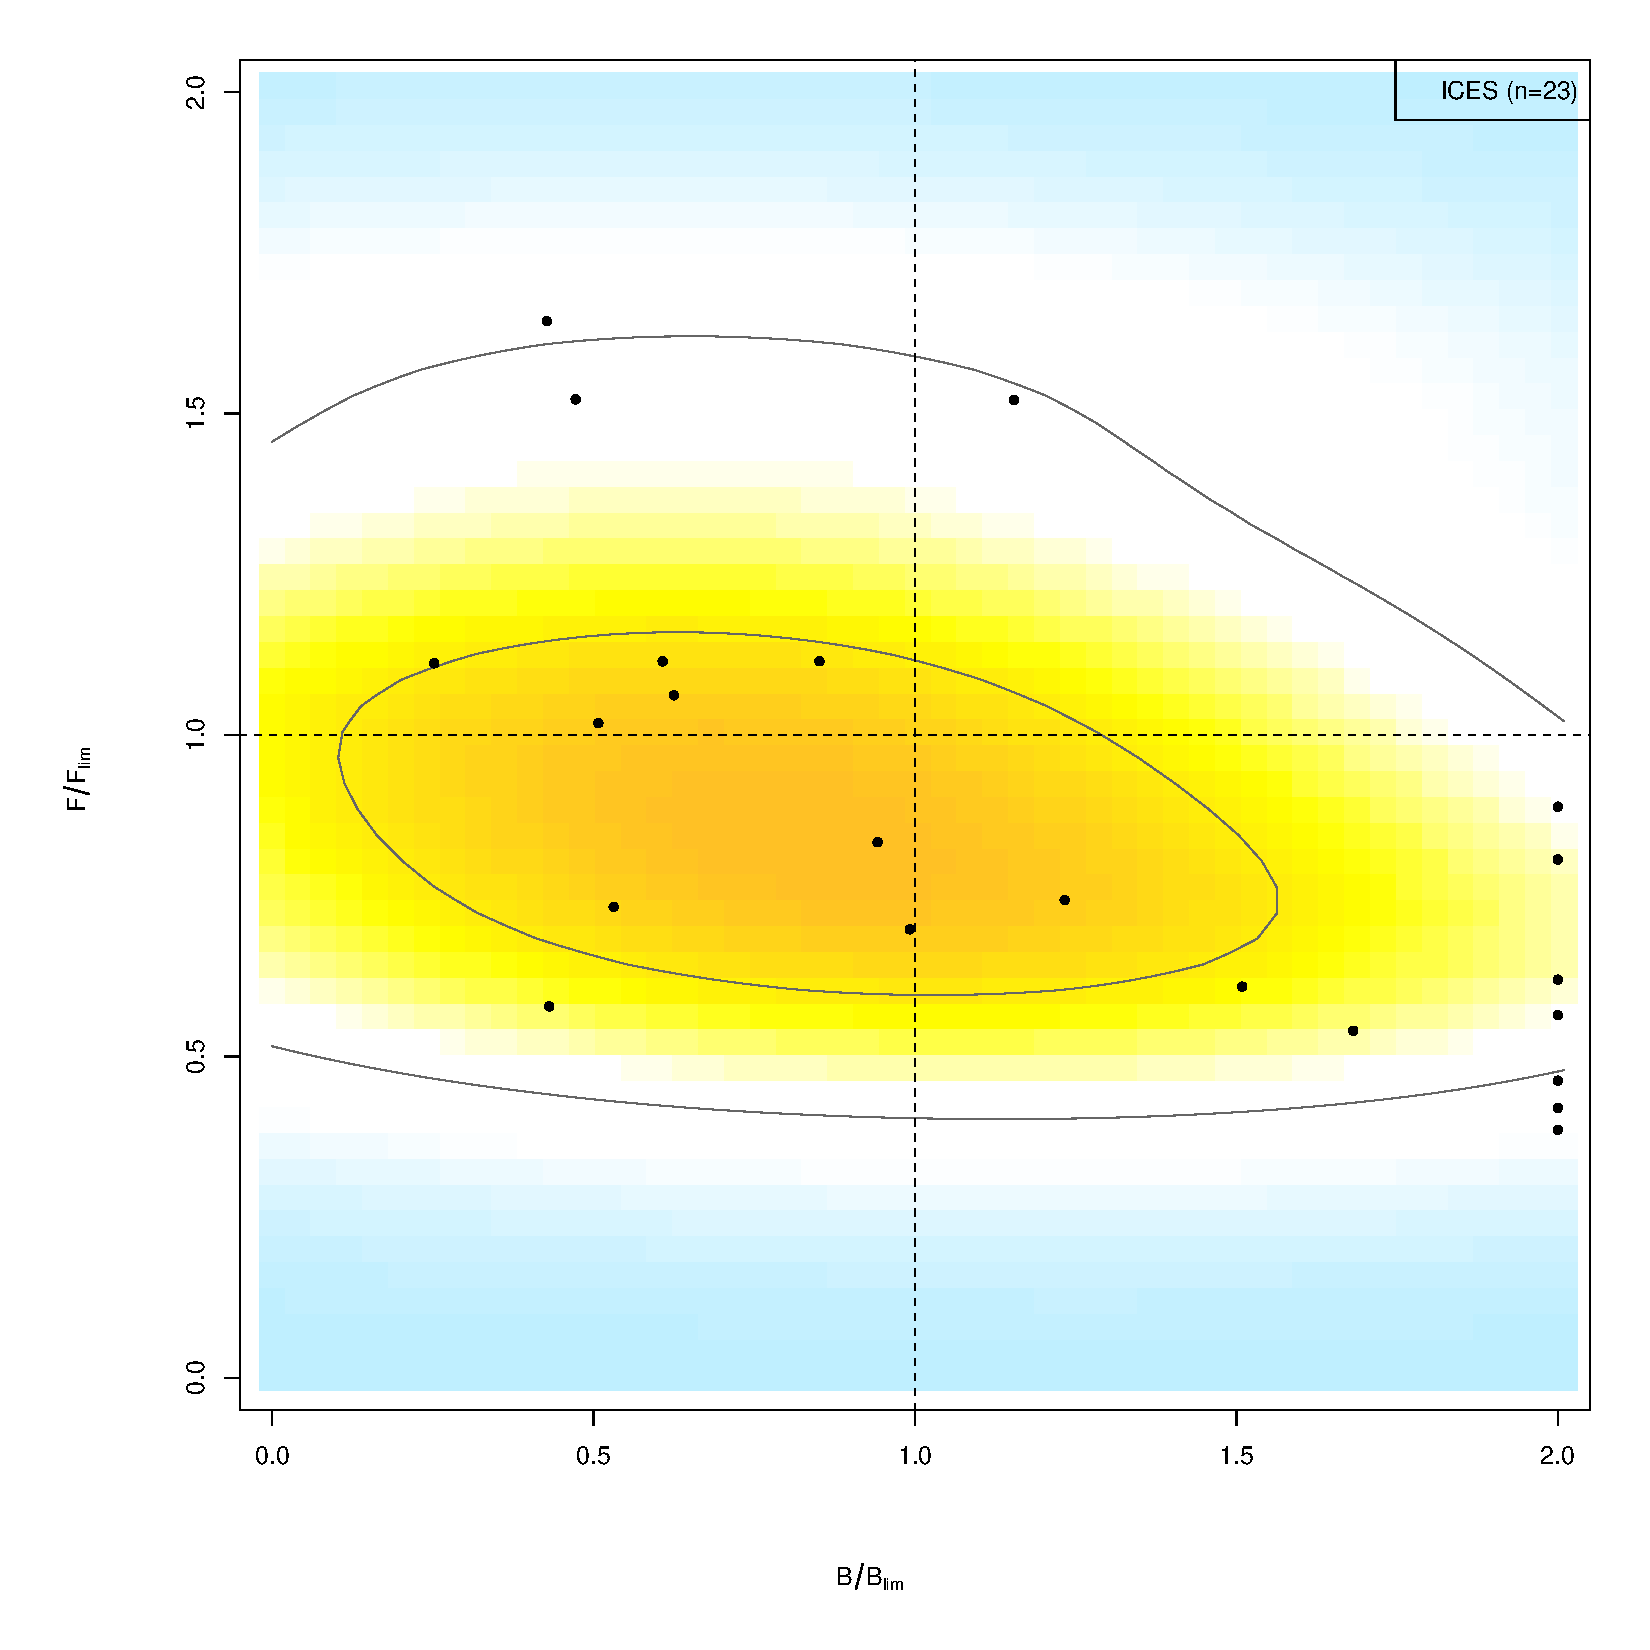
\includegraphics[height=15cm]{/home/srdbadmin/srdb/projects/fishandfisheries/R/PROOFS-final/friedegg-ICES-SSBlim.pdf}
\end{center}
\caption{ ICES SSBlim.}
\label{fig:icesblim}
\end{figure}


%By taxonomy, inverts and fish, demersal and pelagics  (Figure~\ref{fig:group}).
%\begin{figure}
%\begin{center}
%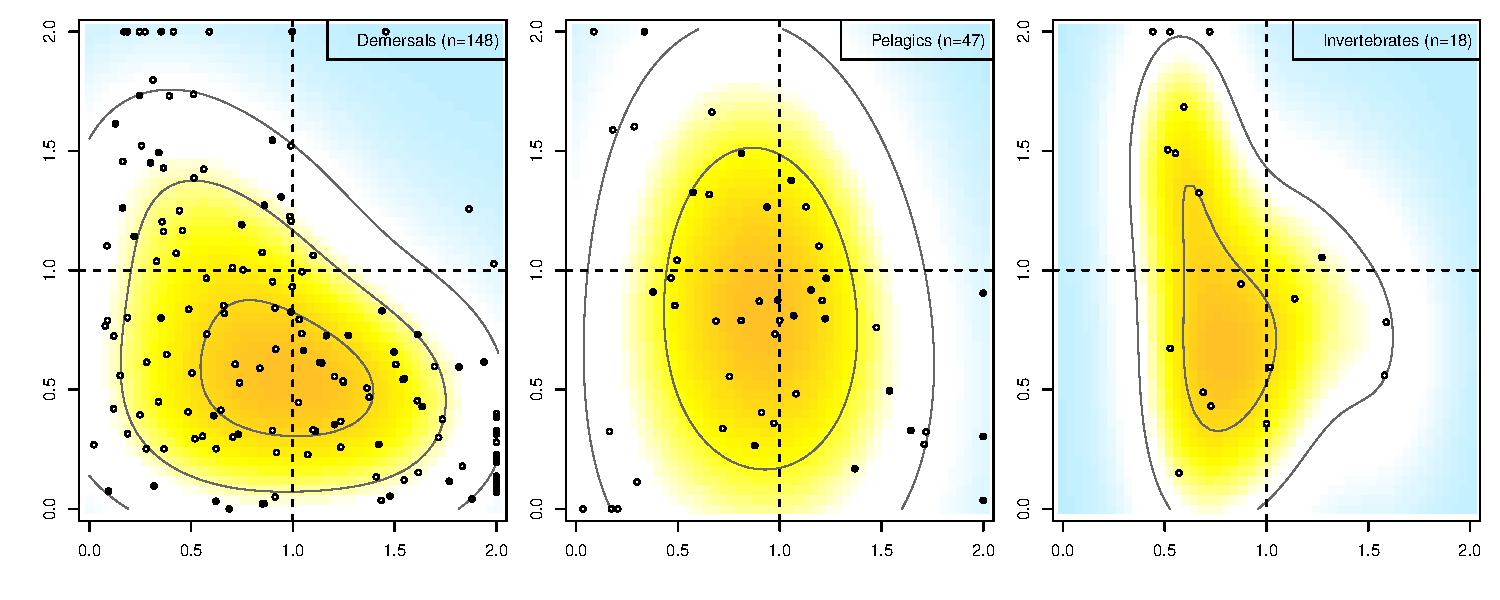
\includegraphics[width=15cm]{/home/srdbadmin/srdb/projects/fishandfisheries/R/PROOFS-final/friedegg-bytaxocategory.pdf}
%\end{center}
%\caption{Invertebrates, demersal fish and pelagic fish.}
%\label{fig:group}
%\end{figure}

\end{document}
